\section{Architettura hardware}
L'infrastruttura computazionale della FitTag Band è incentrata sul System on Chip (SoC) Seeed Studio XIAO nRF52840 Sense Plus.
Questa piattaforma è stata selezionata per la sua elevata densità di integrazione, ospitando nativamente un'unità di misura inerziale (IMU), un ricetrasmettitore per la connettività wireless (Bluetooth Low Energy) e il circuito integrato BQ25101, un controller dedicato alla ricarica e alla gestione in sicurezza della batteria ai polimeri di litio (LiPo).

La rilevazione cinematica del movimento è affidata al sensore LSM6DS3TR-C, un'IMU a 6 gradi di libertà che combina un accelerometro 3D e un giroscopio 3D. Il sensore dispone di una memoria FIFO hardware da $4\,kB$, configurata per l'accumulo temporaneo dei campioni al fine di ridurre la frequenza di risveglio della CPU.
L'interfacciamento con l'unità di elaborazione avviene mediante bus seriale $I^2C$ e sfrutta linee di interrupt hardware dedicate per segnalare in modalità asincrona la disponibilità di nuovi dati, ottimizzando i consumi energetici complessivi.

Il monitoraggio dei parametri vitali è invece deputato al sensore esterno MAX30102. Questa unità integra due diodi emettitori di luce, uno nello spettro del rosso a $660\,nm$ e uno nell'infrarosso a $880\,nm$, accoppiati a un fotorilevatore ad alta sensibilità.
Il modulo comunica con la MCU condividendo il medesimo bus $I^2C$ tramite indirizzamento logico dedicato.

\begin{figure}[h!]
    \centering
    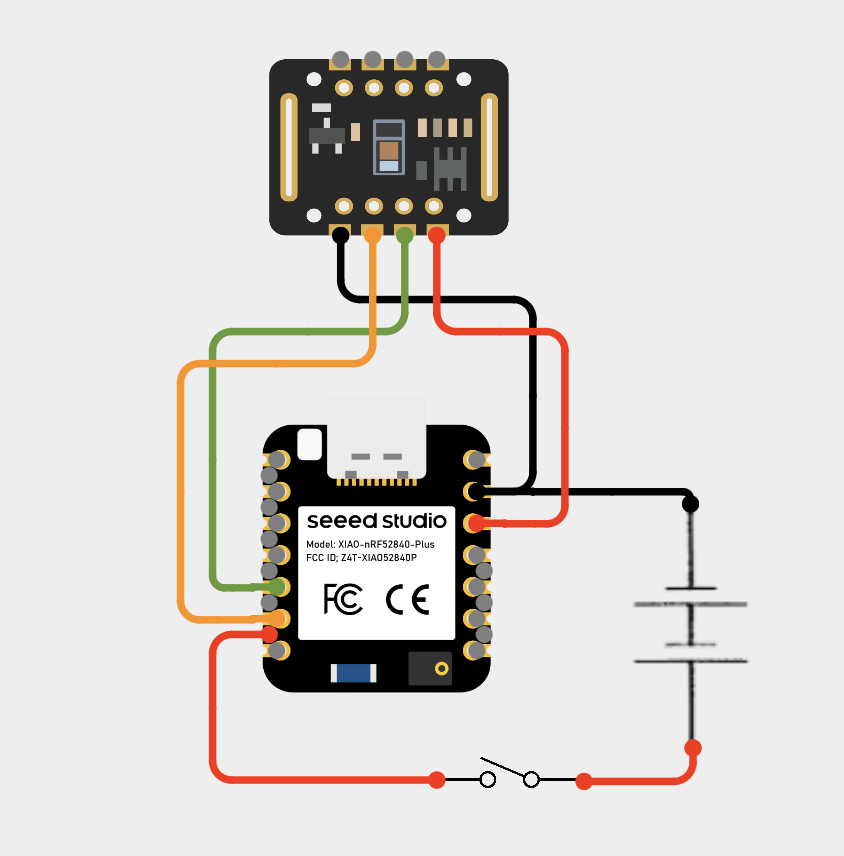
\includegraphics[width=0.5\textwidth]{img/fittag_circuit.png}
    \caption{Schema elettrico del FitTag Band.}
    \label{fig:schema_elettrico}
\end{figure}

\section{Architettura software}
Il firmware del dispositivo è sviluppato in linguaggio C++ sfruttando i vantaggi dell'ambiente integrato PlatformIO e del framework Arduino core per architetture nRF52. L'architettura software è stata progettata come una macchina a stati finiti e si appoggia a librerie specializzate per l'interfacciamento con i sensori e per la gestione del protocollo di comunicazione BLE.

\subsection{La Macchina a Stati Finiti}
La logica di controllo del sistema è orchestrata da una Macchina a Stati Finiti (FSM) che regola in modo deterministico le modalità operative del bracciale.
L'adozione di una FSM consente di implementare politiche attive di risparmio energetico: i sensori e i relativi canali di comunicazione vengono attivati, configurati o posti in modalità di sospensione hardware (sleep mode) esclusivamente quando strettamente richiesto dallo stato corrente.

La FSM è strutturata sui seguenti stati operativi:
\begin{itemize}
    \item \textbf{\texttt{INIT\_STATE}:} Stato transitorio iniziale. Una volta completato il setup, il sistema transita automaticamente verso lo stato di riposo \texttt{IDLE\_STATE}.
    \item \textbf{\texttt{IDLE\_STATE}:} Stato di standby a basso consumo energetico. In questa fase i sensori vengono spenti per preservare la carica della batteria. Questo stato è inoltre lo stato centrale dell FSM, in quanto qualsiasi transizione tra le diverse modalità operative della periferica deve necessariamente transitare attraverso questo stato.
    \item \textbf{\texttt{INFER\_STATE}:} Stato operativo in cui il sistema esegue on-device l'algoritmo di classificazione. L'IMU acquisisce i dati cinematici e li memorizza in un buffer temporaneo per consentire al modello di Machine Learning di stimare l'attività dell'utente in tempo reale.
    \item \textbf{\texttt{DATA\_LOG\_STATE}:} Stato finalizzato alla raccolta dati per l'addestramento offline del classificatore. Il microcontrollore campiona i segnali grezzi di accelerometro e giroscopio a $13\,Hz$ e li trasmette continuamente via BLE verso l'applicazione di raccolta.
    \item \textbf{\texttt{WORKOUT\_STATE}:} Stato attivo di monitoraggio dell'allenamento. In questa modalità vengono abilitati il contapassi hardware integrato nell'IMU e il sensore ottico per la rilevazione del battito cardiaco, calcolando e sincronizzando le metriche prestazionali a intervalli regolari.
    \item \textbf{\texttt{BATT\_LVL\_STATE}:} Stato transitorio deputato alla lettura della tensione della batteria tramite il convertitore analogico-digitale (ADC). La percentuale di carica residua calcolata viene inviata al client BLE prima di far ritornare automaticamente il dispositivo in \texttt{IDLE\_STATE}.
\end{itemize}

\begin{figure}[h!]
    \centering
    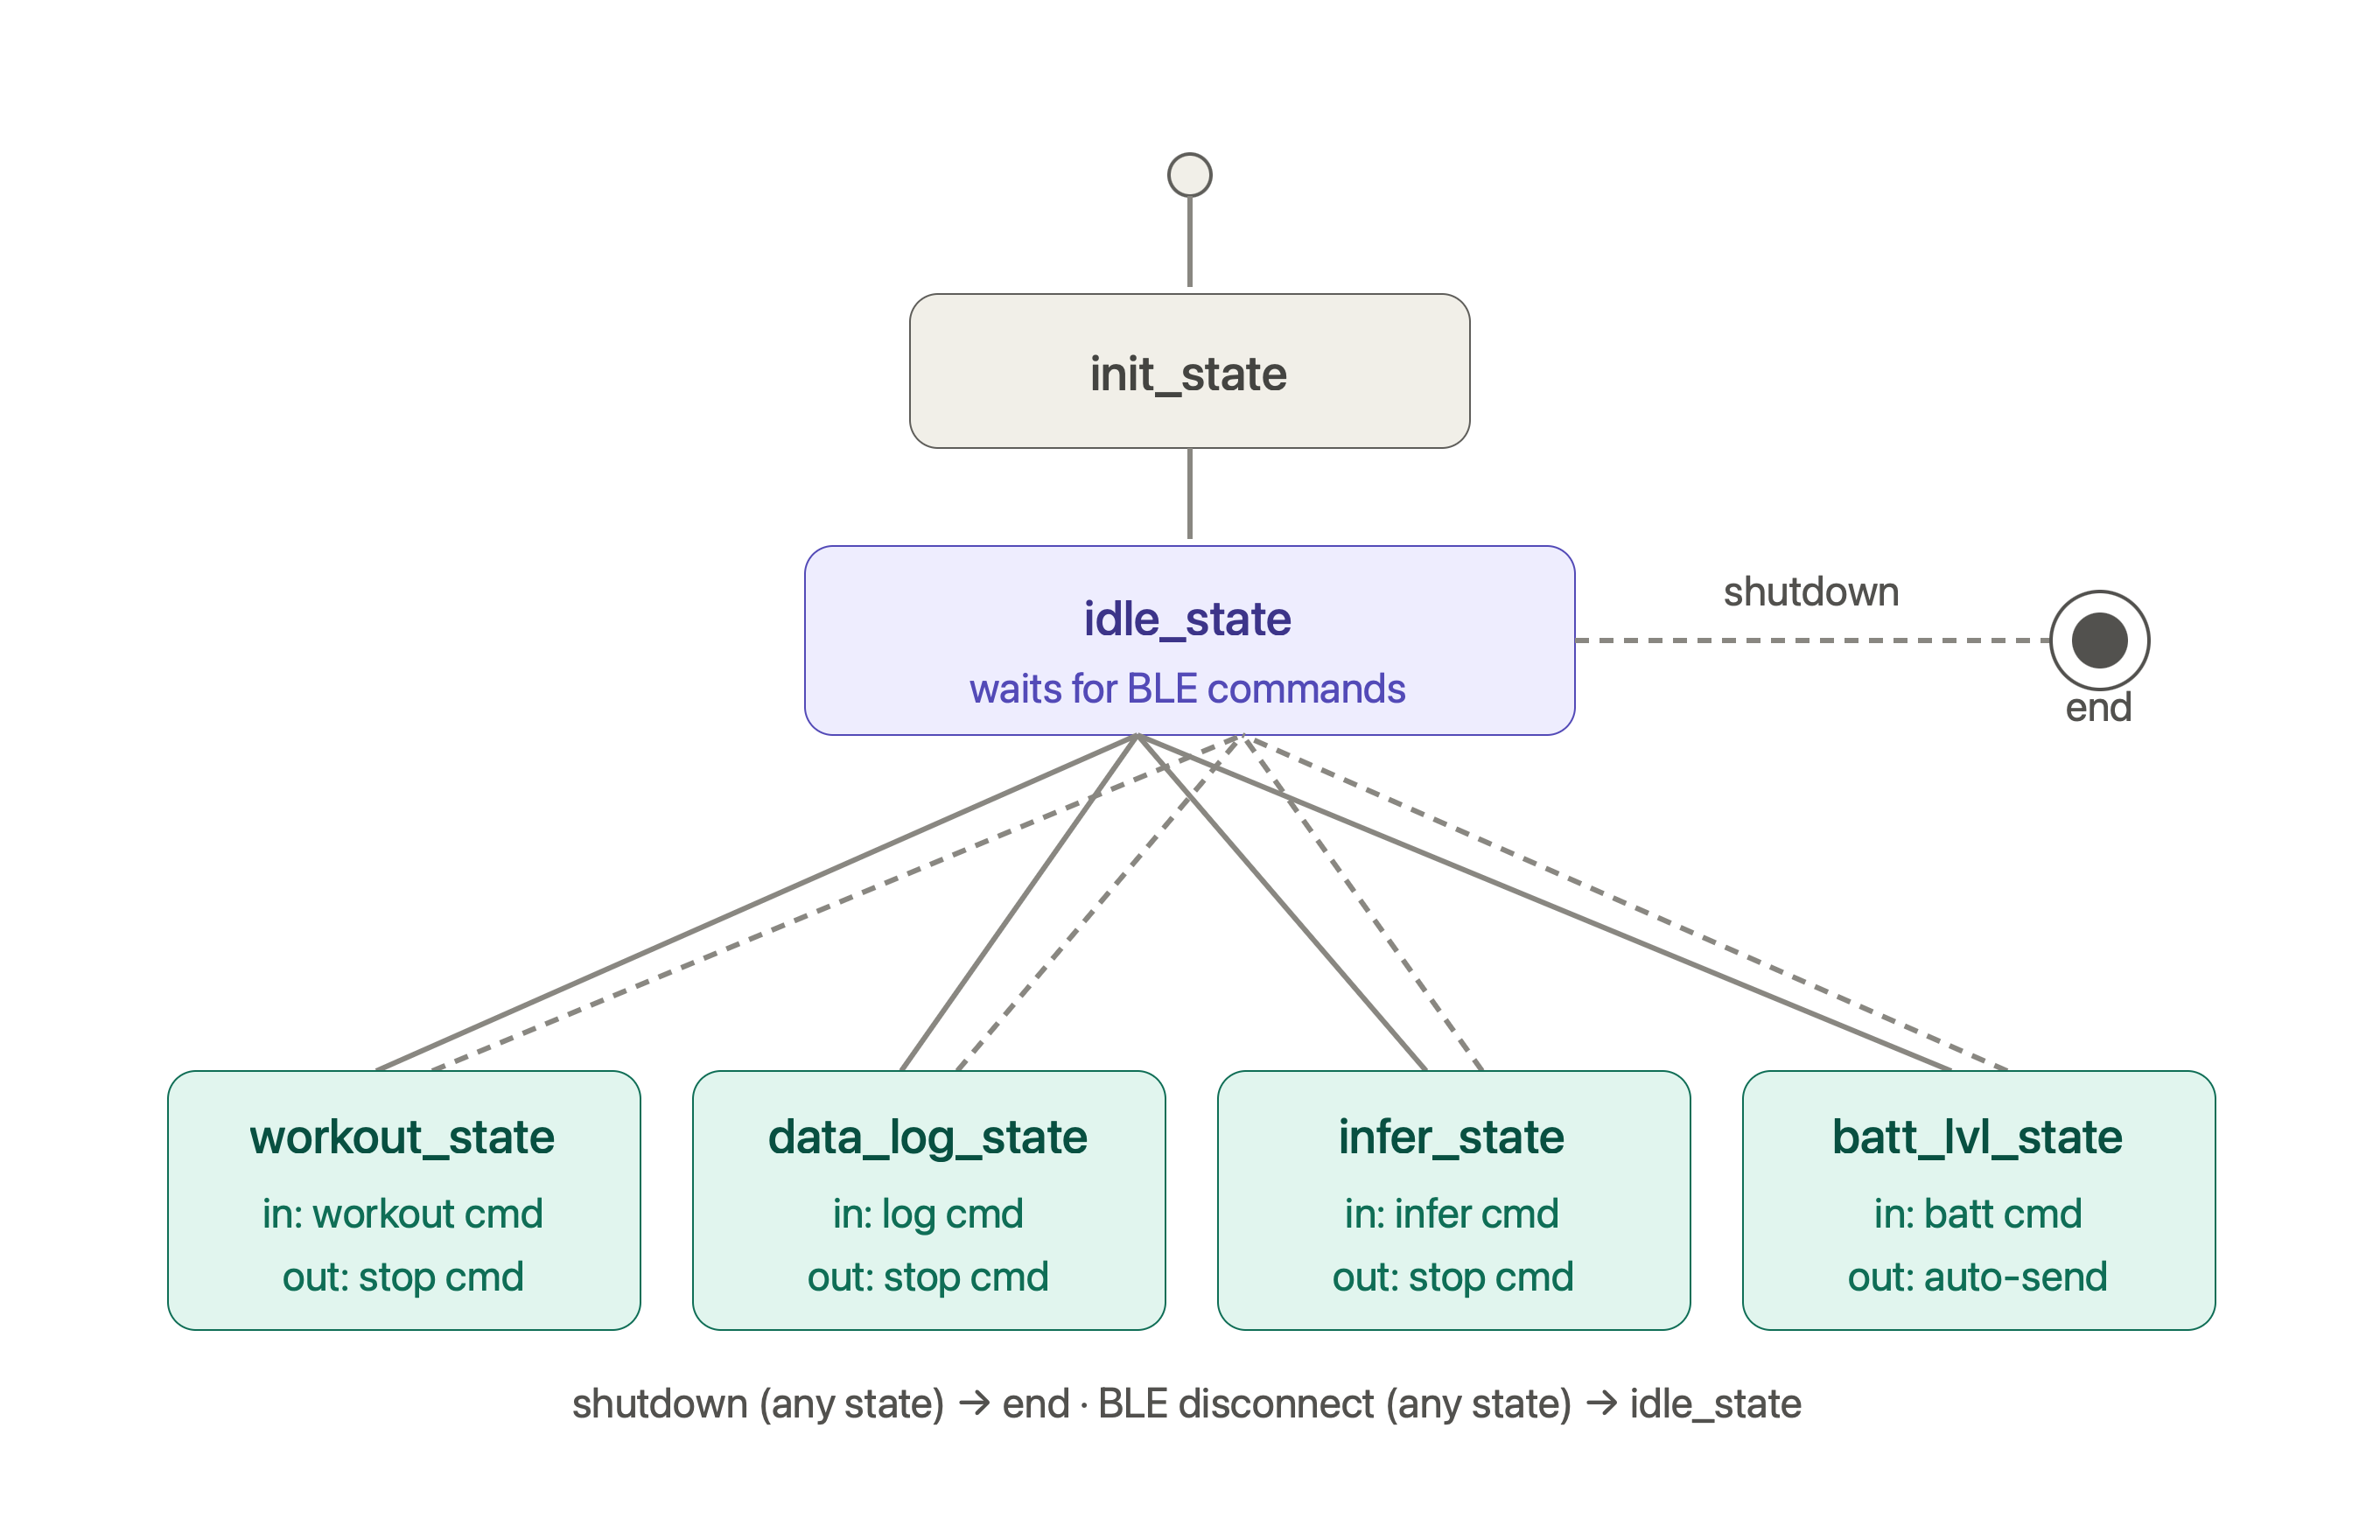
\includegraphics[width=0.55\textwidth]{img/fittag_fsm.png}
    \caption{Diagramma della Macchina a Stati Finiti del FitTag Band.}
    \label{fig:fittag_fsm}
\end{figure}

\subsection{Cose implementate nel codice degne di nota} % TODO: continuare da qua
Per massimizzare l'efficienza energetica, l'architettura è fortemente basata sugli interrupt. Invece di eseguire il \textit{polling} continuo dei sensori, il microcontrollore sfrutta il pin di interrupt \texttt{INT1} dell'LSM6DS3TR-C, configurato per generare un segnale hardware quando la FIFO interna raggiunge una specifica soglia di riempimento. Solo al verificarsi dell'evento la CPU si risveglia, scarica il blocco di dati tramite I2C e li elabora, per poi tornare in uno stato di basso consumo.
Per quanto rigurd i battiti non si usano interrupt pk viene fatto un polling molto lento.

\subsection{GATT BLE}
Il livello di connettività è implementato attraverso uno stack BLE che espone servizi e caratteristiche customizzate. Il dispositivo opera come periferica (\textit{GATT Server}), accettando comandi di controllo sulla caratteristica di scrittura (RX) e trasmettendo in modo asincrono le notifiche (TX) contenenti i log dei sensori, le metriche sportive e le predizioni del modello algoritmico.

\section{Modello ML}
La capacità di \textit{Human Activity Recognition} (HAR) del bracciale è resa possibile dall'implementazione \textit{on-device} di un classificatore ad albero, specificamente un \textit{Random Forest}, ottimizzato per l'esecuzione su sistemi embedded con risorse limitate (TinyML).

Il firmware applica un approccio a finestra temporale scorrevole (\textit{Sliding Window}) sui dati grezzi di accelerometro e giroscopio. Per campionamenti a 13 Hz, il sistema accumula dati in una finestra di 5 secondi (65 campioni). Per garantire una reattività ottimale mantenendo un contesto storico sufficiente, la finestra avanza con uno scivolamento (\textit{overlap}) di 2 secondi (26 campioni), permettendo di generare una nuova predizione regolarmente senza perdere ciclicità nel movimento.

Da ogni finestra temporale viene estratto un vettore di caratteristiche (\textit{features}) calcolando la media e la deviazione standard per ciascuno dei 6 assi inerziali. Il vettore risultante di 12 elementi in virgola mobile viene elaborato dal \textit{Random Forest}, il quale attraversa le diramazioni logiche generate in fase di addestramento e restituisce la classe di attività riconosciuta mediante un meccanismo di maggioranza sui voti degli alberi decisionali.